\documentclass[a4paper,10pt]{article}
\usepackage[utf8]{inputenc}
\usepackage[english]{babel}
\usepackage{float}
\usepackage{graphicx}
\usepackage{caption}
\usepackage{subcaption}
\usepackage{amsmath}

%opening
\title{Deep convolutional networks for protein fold recognition}
\author{}

\begin{document}

\maketitle

\begin{abstract}

\end{abstract}

\section{Introduction}
Proteins are the cogs of the cell machinery. In order to understand responses of a cell to the external stimuli given their internal state, we
have to be able to predict the function of the proteins expressed in a cell. The current paradigm dictates that the function of a protein is determined
mainly by its structure and its interactions with other molecules present in a cell. Therefore the problem of a protein structure prediction 
(protein folding) is one of the limiting factors in the progress of biology.

Recent progress in protein folding relies mostly on the increasing computing capacity. Current methods can generate thousands of 
candidate structures (decoys) given its sequence. Hence the selection of the most viable candidates comes to the forefront as the limiting 
factor in solving the protein folding problem. 

Deep learning (DL) is a popular  approach in the field of machine learning, which recently gained considerable interest in the research community \cite{lecun2015deep}, 
particularly in computer vision and image recognition. Unlike previous ‘shallow’ approaches, DL tries to learn hierarchical representation of the 
data in hand. It alleviates the need for feature extraction that constituted the bulk of the work done by researchers. 

Recently, DL was applied to biological data and yielded remarkable results in the human splicing code prediction \cite{xiong2015human}, 
identification of DNA- and RNA-binding  motifs \cite{alipanahi2015predicting} and predicting the effects of non-coding DNA variants at single nucleotide polymorphism 
precision \cite{zhou2015predicting}. These successes have one thing in common: they do not introduce any features between the raw data and the deep learning model. 

Deep learning methods were also applied in the field of structure quality assessment \cite{}. In particular, DeepQA \cite{} used 9 scores from other QA estimators and 
7 physico-chemical feature estracted from a structure as the input features to the deep boltzman machine \cite{}. In the DL-PRO algorithm \cite{}, authors first compute 
contact maps of the decoys and compress them using PCA. The vectors from PCA are then fed into an autoencoder to predict the score of the decoy. The authors that apply the 
deep learning methods use them as the ordinary 'shallow' classifiers. Therefore they do not get all the advantages these new techniques offer.

In this paper we show, that deep convolutional networks with the raw atomic density input can outperform conventional methods that mainly rely on the feature engineering.

\section{Materials and Methods}
\subsection{Datasets}
To train and assess our method we used the two datasets of protein decoys: 3DRobot dataset \cite{} and CASP datasets \cite{}. The decoys in 3DRobot dataset 
were generated using free fragment assembly followed by optimization of hydrogen bonding and compactness of the decoys. It contains 200 structures with 300 decoys
for each. They have near-even distribution of root mean squared deviation with respect to the corresponding native structure. This dataset was used to tune the 
hyperparameters of the model and the training procedure.
The CASP datasets were used to asses the quality of the predictions. We took the datasets from CASP7 - CASP10 as the training set and the CASP11 dataset as the test set.
We also generated the second version of the CASP training and test sets by optimizing sidechains with SCWRL program \cite{}.

\subsection{Input and Model}
\begin{figure}[H]
    \centering
    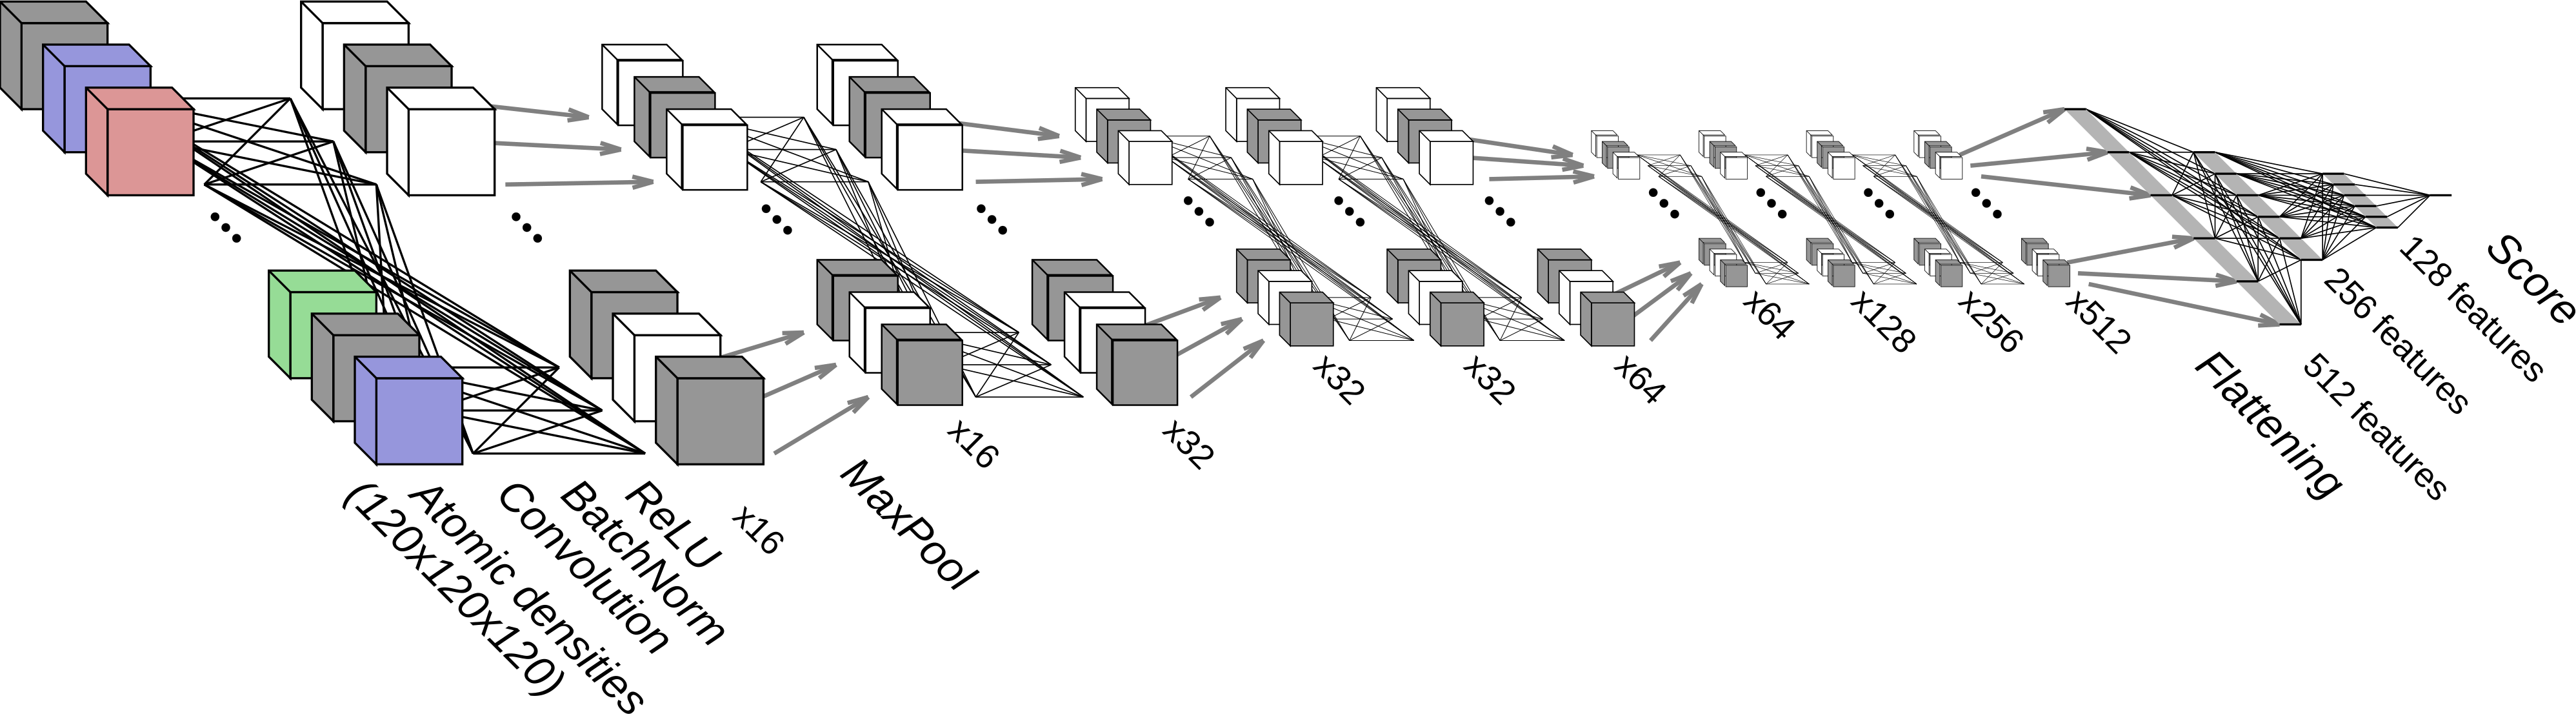
\includegraphics[width=\linewidth]{../scripts/Figures/ConvnetDiagram/ConvnetDiagramV1.png}
    \caption{The schematic representation of the convolutional neural network architecture used in this work.}
    \label{Fig:CNNModel}
\end{figure}
The schematic representation of the model architecture is shown on the Fig \ref{Fig:CNNModel}. It is comprised of three blocks of alternating convolutional, 
volumetric batch normalization and ReLU layers and three 
fully connected layers with ReLU nonlinearities. The final output of the network is a single number, that is interpreted as a score of an input structure.
The input of the model is the density maps of atom types in a structure. We used 11 types of atoms shown in the Table \ref{Tbl:atomTypes}. 
Each atom type was projected on the corresponding grid and served as an input of the model. The density of an atom was modeled using the function: 
$$
\rho(r) =  \begin{cases}
               e^{-\frac{r^2}{2}}&r\leq 2.0\AA~\\
               0                 &r>2.0\AA~\\
            \end{cases}
$$
\begin{table}[H]
\begin{center}
\begin{tabular}{ c | l | l }
    
    Type & Description & Atoms \\
    \hline
    1 & Sulfur containing atoms & CYSSG, METSD, MSESE \\ \hline
    2 & Amide nitrogens & ASNND2, GLNNE2, backbone N \\ \hline
    3 & Aromatic nitrogens & HISND1, HISNE2, TRPNE1 \\ \hline
    4 & Guanidine nitrogens & ARGNH1, ARGNH2, ARGNE \\ \hline
    5 & Nitrogen with three hydrogens & LYSNZ \\ \hline
    6 & Carboxyl oxygen & ACEO, ASNOD1, GLNOE1, backbone O \\ \hline
    7 & Oxygen in hydroxyl group & SEROG, THROG1, TYROH \\ \hline
    8 & Oxygen in carboxyl group and terminus oxygen & ASPOD1, ASPOD2, GLUOE1, GLUOE2, \\
     & &  O-terminal, OT2-terminal, OXT-terminal \\ \hline
    9 & Sp2 carbon & ARGCZ, ASPCG, GLUCD, ACEC, \\
     & & ASNCG, GLNCD, backbone C\\ \hline
    10 & Aromatic carbon & HISCD2, HISCE1, HISCG, PHECD1 \\
     & & PHECD2, PHECE1, PHECE2, PHECG \\ 
     & & PHECZ, TRPCD1, TRPCD2, TRPCE2 \\
     & & TRPCE3, TRPCG, TRPCH2, TRPCZ2 \\
     & & TRPCZ3, TYRCD1, TYRCD2, TYRCE1 \\
     & & TYRCE2, TYRCG, TYRCZ \\ \hline
    11 & Sp3 carbon & ALACB, ARGCB, ARGCG, ARGCD \\
     & & ASNCB, ASPCB, GLNCB, GLNCG\\
     & & GLUCB, GLUCG, HISCB, HISCB \\
     & & ILECB, ILECD1, ILECG1, ILECG2 \\
     & & LEUCB, LEUCD1, LEUCD2, LEUCG \\
     & & LYSCB, LYSCD, LYSCG, LYSCE \\
     & & METCB, METCE, METCG, MSECB \\
     & & MSECE, MSECG, PHECB, PROCB \\
     & & PROCG, PROCD, SERCB, THRCG2 \\
     & & TRPCB, TYRCB, VALCB, VALCG1 \\
     & & VALCG2, ACECH3, THRCB, CYSCB \\
     & & backbone CA \\ \hline
    
\end{tabular}
    
    \caption {Atom types used in this work. In the atom notation the first three letters are the name of an aminoacid and the rest is 
    the atom name in the PDB format \cite{}}.
    \label{Tbl:atomTypes}
\end{center}
\end{table}

\subsection{Loss functions}
We evaluated two scoring functions: linear regression and ranking scoring function. Let a decoy representation be denoted as $x_i$ and therefore the output
of the network on this decoy will be $f(x_i)$. Next, let $y_{ij}$ be the ordering coefficient of the two decoys we pick: 
$$
y_{ij} = \begin{cases}
               1& gdtts_i \leq gdtts_j \\
               -1& gdtts_i > gdtts_j \\
            \end{cases}
$$
Here $gdtts_i$ is the GDT-TS score of the $i$-th decoy. In principle, any target function can be chosen. We also tried RMSD and TM-Score functions, but the results for
these two scoring schemes are not presented in this paper. After we explained notation we can define the pairwise ranking scoring function:

$$ L_{ij} = w_{ij} \cdot \max \left[ 0, 1 - y_{ij} \left( f \left( x_i \right) - f \left( x_j \right) \right) \right] $$

the term $w_{ij}$ represents an example weight:

$$
w_{ij} = \begin{cases}
               1& \left| gdtts_i - gdtts_j \right| > threshold \\
               0& otherwise \\ 
            \end{cases}
$$

where the $threshold$ we define manually. If the two decoys are too similar, we avoid scoring them against each other during the training, because it introduces 
the noise into the gradient and prevents optimization. We observed that the noisy gradient results in the final model, that scores all the decoys equally.


During the training procedure we load several decoys (batch) into memory and evaluate the model on them. Afterwards, we compute the average loss for the batch:
$$ L = \frac{1}{N} \sum_{i=1,j=1, i \neq j}^{M} L_ij $$ 
where $N$ is the number of pairs of decoys with the $w_{ij} > 0$ and $M$ is the number of decoys in a batch.

The linear regression loss function is also defined on a batch of decoys. TODO.

\subsection{Optimization and dataset sampling}
The optimization procedure of deep convolutional networks usually is stochastic: the function value and gradient is estimated on a small subset (batch) of all the training 
examples. We used the batch of size 10 due to memory limitations. The optimization algorithm we used was Adam \cite{} with hyper-parameters shown in Table \ref{Tbl:optParams}. 

The dataset was sampled in the following way: first we chose a random protein from the dataset, then we sample decoys of this protein. The procedure is repeated for all the 
proteins in a dataset. One pass through all the proteins in a dataset is called epoch. 
The decoys are sampled in a homogeneous way: we divide all the decoys into $M$ clusters by the value of GDT-TS score. Precisely, the decoy $i$ belongs to the cluster  
number $ \left[ \frac{\max(gdtts) - gdtts_i}{\max(gdtts) - \min(gdtts)} \right] + 1$, where $\max(gdtts)$ and $\min(gdtts)$ are computed for all the decoys of 
the chosen protein. If there are empty clusters, then we take secon decoys from each non-empty and so on until we filled the batch. At the end of each epoch we randomly
shuffle the order of protein and the order of decoys in each cluster.

We also found that decreasing $threshold$ in the example weights $w_{ij}$ during training is beneficial. The exact schedule for this parameter during the training procedure 
is shown in the Table \ref{Tbl:optParams}.

\begin{table}[H]
\begin{center}
\begin{tabular}{ l | l }
    
    Parameter & Value \\
    \hline
    $L_1$ regularization coefficient & $1 \cdot 10^-5$ \\ \hline
    Learning rate & $0.5 \cdot 10^-4$ \\ \hline
    Number of epochs & 150 \\ \hline
    GDT-TS threshold & epoch 1 : $0.3$ \\ 
                     & epoch 20 : $0.2$ \\ 
                     & epoch 40 : $0.1$ \\ 
                     & epoch 80 : $0.0$ \\ \hline
\end{tabular}
    
    \caption {Optimization parameters and GDT-TS threshold curriculum.}
    \label{Tbl:optParams}
\end{center}
\end{table}


\section{Results}
We evaluated our algorithm using the correlation coefficients, Z-score and loss criterions. The correlation coefficents were computed between the score of 
our model and GDT-TS metric for all the decoys of each protein in the CASP11 test dataset and then averaged. The Z-score is the deviation of the score of 
the best decoy for a certain protein and average decoy score for this protein:
$$ 
Z-score = \frac{f( argmin(gdtts(x_i)) ) - <f(x)>}{std.dev.f(x)}
$$ 
the best decoy is the one with the lowest GDT-TS score. 
The loss criterion is the deviation of the GDT-TS of the best decoys for a protein from the GDT-TS score of the decoy with the lowest score:
$$ 
Loss = | max_i( gdtts_i ) - gdtts( argmin(f(x_i) ) |
$$ 

Table \ref{} shows the comparisson of our model with the state of art methods used for the decoy quality assessement. We used CASP11 dataset to measure the 
characteristics. As we mentioned before we generated two versions of this dataset: the raw dataset and the one where each decoy sidechains were optimized with 
the help of SCWRL program \cite{}. We also evaluated the performance of our ranking algorithm on the proteins on different size separately. These results are shown 
in the Table \ref{}. 

\begin{table}[H]
\begin{center}
\begin{tabular}{ c | c | c | c | c }
    
    QA method & Mean loss & Mean Pearson corr. & Mean Spearmann corr. & Mean Kendall corr. \\
    \hline
    CNN     & & & & \\ \hline
    ProQ2   &0.090 &0.643 &0.506 &0.379 \\ \hline
    Qprob   &0.097 &0.631 &0.517 &0.389 \\ \hline
    Dope    &0.111 &0.542 &0.416 &0.316 \\ \hline
    RWplus  &0.135 &0.536 &0.433 &0.433 \\ \hline
\end{tabular}
    
    \caption {Results of our method and other state-of-art quality assessment programs on CASP11 dataset stage 1.}
    \label{Tbl:optParams}
\end{center}
\end{table}

\begin{table}[H]
\begin{center}
\begin{tabular}{ c | c | c | c | c }
    
    QA method & Mean loss & Mean Pearson corr. & Mean Spearmann corr. & Mean Kendall corr. \\
    \hline
    CNN     & & & & \\ \hline
    ProQ2   &0.058 &0.372 &0.366 &0.256 \\ \hline
    Qprob   &0.068 &0.381 &0.387 &0.272 \\ \hline
    Dope    &0.077 &0.304 &0.324 &0.228 \\ \hline
    RWplus  &0.084 &0.295 &0.314 &0.220 \\ \hline
\end{tabular}
    
    \caption {Results of our method and other state-of-art quality assessment programs on CASP11 dataset stage 2.}
    \label{Tbl:optParams}
\end{center}
\end{table}


\section{Discussion}

\bibliography{citations.bib}{}
\bibliographystyle{plain}


\end{document}
